\documentclass[tikz,border=7pt]{standalone}
\usepackage[T1]{fontenc}
\usetikzlibrary{arrows.meta}
\begin{document}
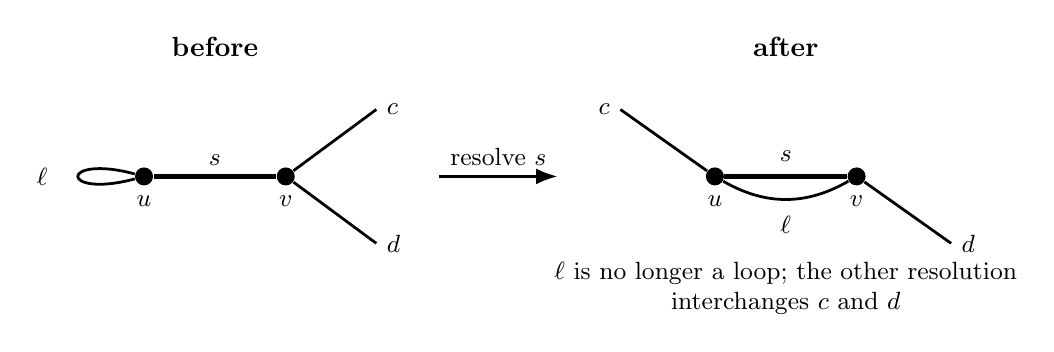
\begin{tikzpicture}[
  vertex/.style={circle,fill=black,inner sep=2.3pt},
  edge/.style={line width=1pt},
  central/.style={line width=1.5pt},
  arrow/.style={-{Latex[length=2.7mm]},line width=.9pt},
  every node/.style={font=\small}
]
  \node[font=\bfseries] at (-3.8,1.65) {before};
  \node[vertex,label=below:$u$] (u0) at (-4.7,0) {};
  \node[vertex,label=below:$v$] (v0) at (-2.9,0) {};
  \draw[edge] (u0) edge[loop left,min distance=10mm]
    node[left=.25cm] {$\ell$} (u0);
  \draw[central] (u0)--(v0) node[midway,above] {$s$};
  \draw[edge] (v0)--(-1.75,.85) node[right] {$c$};
  \draw[edge] (v0)--(-1.75,-.85) node[right] {$d$};

  \draw[arrow] (-.95,0)--(.55,0) node[midway,above] {resolve $s$};

  \node[font=\bfseries] at (3.45,1.65) {after};
  \node[vertex,label=below:$u$] (u1) at (2.55,0) {};
  \node[vertex,label=below:$v$] (v1) at (4.35,0) {};
  \draw[central] (u1)--(v1) node[midway,above=.05cm] {$s$};
  \draw[edge] (u1) to[bend right=30]
    node[midway,below=.08cm] {$\ell$} (v1);
  \draw[edge] (u1)--(1.35,.85) node[left] {$c$};
  \draw[edge] (v1)--(5.55,-.85) node[right] {$d$};
  \node[align=center] at (3.45,-1.42)
    {$\ell$ is no longer a loop; the other resolution\\
     interchanges $c$ and $d$};
\end{tikzpicture}
\end{document}
